\subsection{Bestimmung der Schallgeschwindigkeit mithilfe von Mikrofonen}
Die Schallgeschwindigkeit lässt sich durch die Bestimmung der Steigung zwischen zwei Mikrofonabstandsdifferenzen ermitteln. Hierzu wird eine Ausgleichsgerade, wie in Abbildung \ref{fig:aufgabe3} dargestellt errechnet.\footnote{Berechnung durch Origin} Die Steigung entspricht der Schallgeschwindigkeit.\\
Der statistische Fehler der Zeit wird auf $\pm \unit[20]{\mu s}$ geschätzt (Ableseungenauigkeit), es ergibt sich also ein Fehler der Differenz von $\pm \unit[28]{\mu s}$. Der statistische Fehler für die Einstellung auf der Skala beträgt halbe Strichgröße, der Fehler für den Abstand beträgt also $\unit[0.07]{cm}$. Durch die lineare Regression sind diese Fehler allerdings nicht von Bedeutung (konstant, daher keine Gewichtung). Für die Steigung $c_S$ der Ausgleichsgerade erhalten wir folgenden Wert:
\begin{equation}
c_s = \unit[(0.03495 \pm 0.00028)]{\frac{cm}{\mu s}} = \unit[(349.5 \pm 2.3)]{\frac{m}{s}}
\end{equation}
Dieser Wert weicht (auch außerhalb des Fehlerbereichs) leicht von Literaturwerten bei ähnlichen Bedingungen ab.\footnote{David R. Lide: Handbook of Chemistry and Physics, CRC Press, 85. Auflage, Seite 14-41}
Grund hierfür sind wahrscheinlich systematische Fehler der Messgeräte und/oder bei der Messung (Mikrofon, Oszilloskop), die uns leider nicht bekannt sind.\\
Die Ausgleichsgerade läuft mit großer Wahrscheinlichkeit nicht durch den Ursprung, da nur die Differenz des Abstandes der Mikrofone genau bestimmt werden kann, nicht aber der Abstand der Mikrofone.

\begin{figure}
\begin{center}
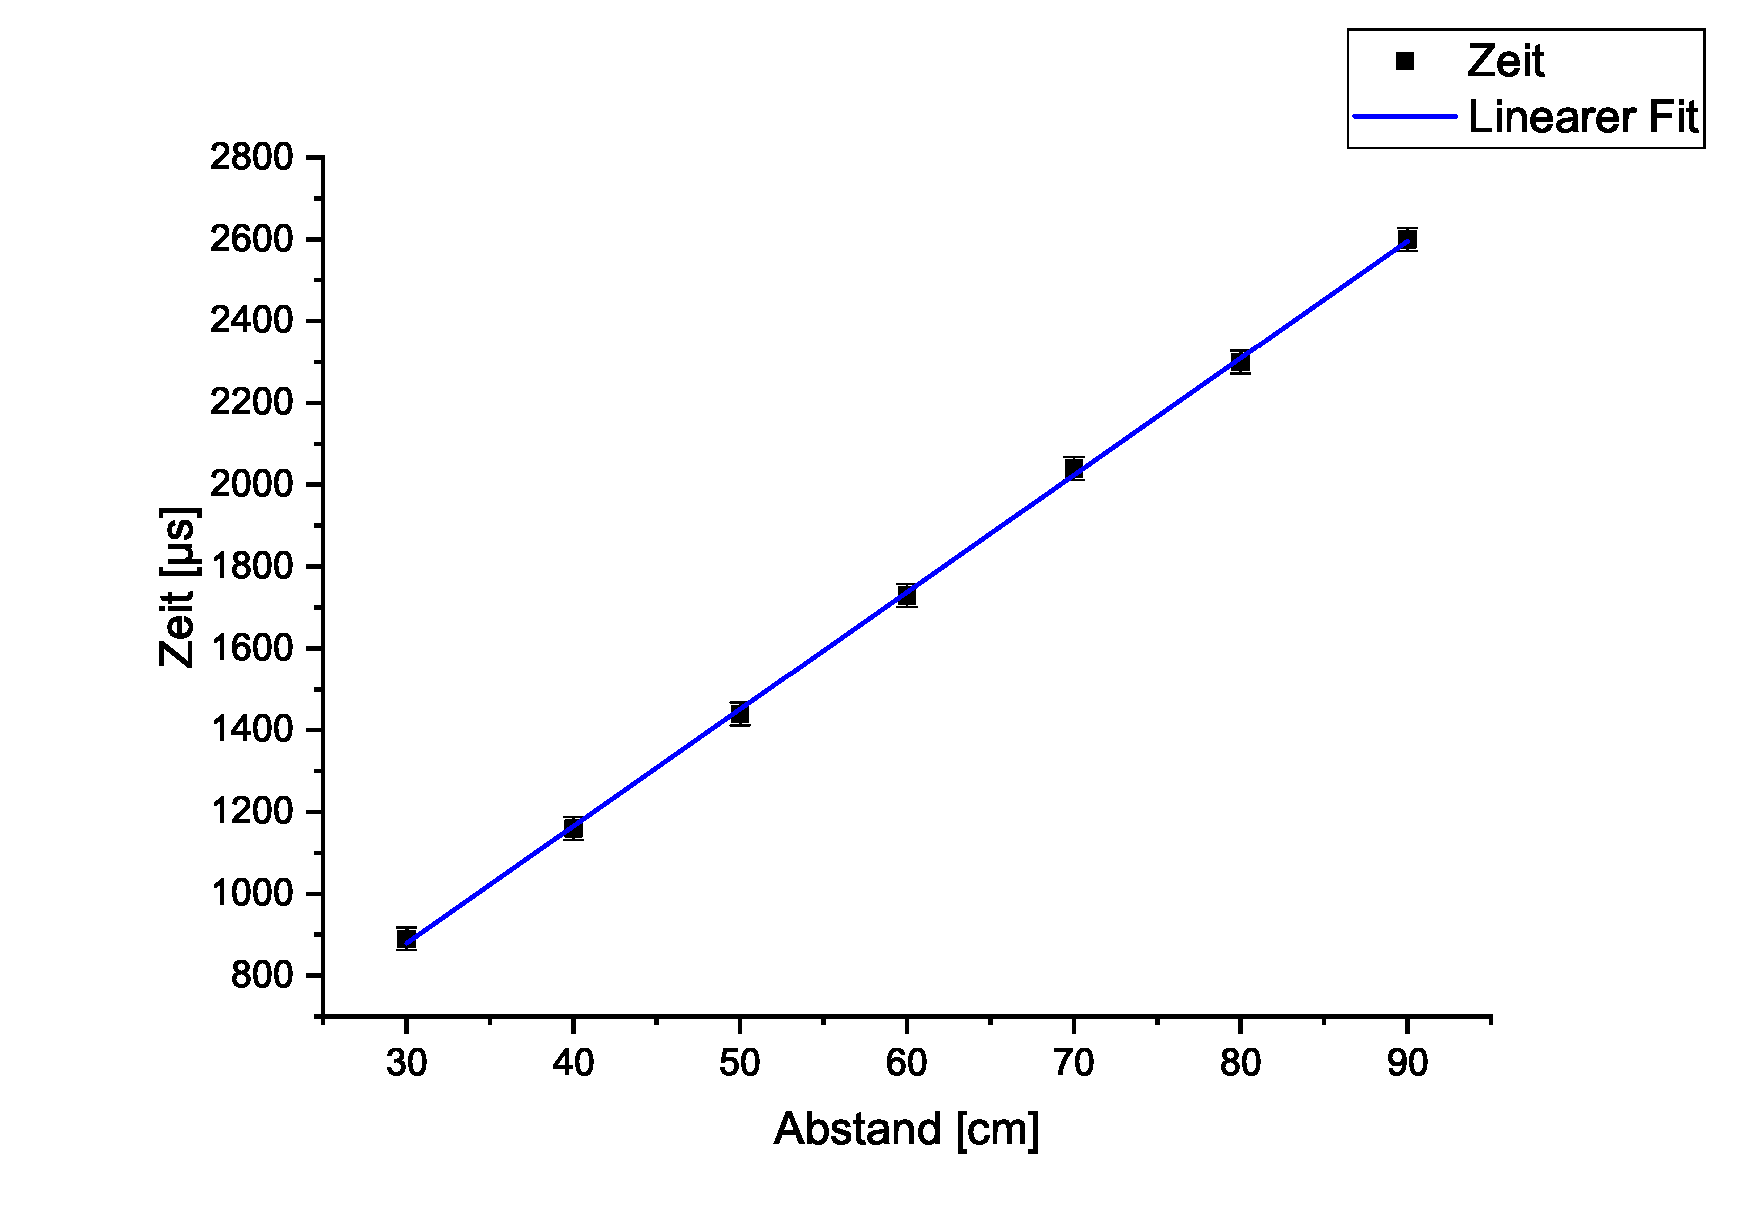
\includegraphics[width=0.6\textwidth]{Bilder/aufgabe3.eps}
\caption{Berechnung der Schallgeschwindigkeit}
\label{fig:aufgabe3}
\end{center}
\end{figure}